% Kapitel 3.3 -- Europäische Union


\subsection{Europäische Union}

Die Europäische Union (EU) verfolgt bei Kryptowährungen keinen Ansatz, bei dem private Krypto-Assets als gesetzliches Zahlungsmittel eingeführt werden. Der Begriff Krypto-Assets bezeichnet digitale Darstellungen von Werten oder Rechten, die elektronisch übertragen und gespeichert werden können \cite{MiCA2023}. Die EU behandelt solche Vermögenswerte nicht als Ersatz für den Euro, sondern als regulierte Finanz- und Vermögenswerte. Damit unterscheidet sich der europäische Ansatz von El Salvador, wo Bitcoin gesetzliches Zahlungsmittel wurde, und von Dubai, wo ein regulierter Krypto-Standort aufgebaut wird.

Für die Forschungsfrage ist der europäische Fall besonders relevant. Er zeigt, dass Kryptowährungen nicht nur wegen technischer Eigenschaften begrenzt bleiben. Entscheidend sind auch staatliche Kontrolle, Regulierung, Verbraucherschutz und gesellschaftliches Vertrauen.

\subsubsection{Warum die EU Kryptowährungen nicht als Zahlungsmittel eingeführt hat}

Ein zentraler Grund ist der Schutz des staatlichen Geldsystems. In der Eurozone liegt die Geldpolitik bei der Europäischen Zentralbank (EZB). Würden private Kryptowährungen eine zentrale Rolle als Zahlungsmittel übernehmen, könnten geldpolitische Steuerung, Finanzstabilität und staatliche Kontrolle über Zahlungsströme geschwächt werden. Die EU behandelt Kryptowährungen deshalb nicht als Ersatz für den Euro, sondern als Vermögenswerte mit besonderen Risiken.

Hinzu kommt der Verbraucherschutz. Kryptowährungen sind für viele Nutzer schwer verständlich, ihr Wert kann stark schwanken, und Anbieter im Kryptomarkt waren vor der europäischen Regulierung nicht einheitlich beaufsichtigt. Die wichtigste regulatorische Antwort ist die \emph{Markets in Crypto-Assets Regulation} (MiCA; deutsch: EU-Verordnung über Märkte für Kryptowerte). MiCA ist keine Kryptowährung, sondern ein Rechtsrahmen der EU für Krypto-Assets und Krypto-Dienstleister. Die Verordnung regelt unter anderem Transparenzpflichten, Zulassung, Aufsicht, Verbraucherschutz und Marktintegrität \cite{MiCA2023}.

Auch die EZB bewertet Bitcoin als Zahlungsmittel kritisch. Bindseil und Schaaf argumentieren im Blog der EZB, dass Bitcoin außerhalb bestimmter Nischen kaum für Zahlungen genutzt werde und weiterhin Probleme wie hohe Kursschwankungen, technische Grenzen und Umweltbelastungen aufweise \cite{Bindseil2024}. Diese Position erklärt, warum private Kryptowährungen in der EU nicht die Rolle von öffentlichem Geld erhalten.

\subsubsection{Prozess: MiCA-Verordnung und digitaler Euro}

MiCA schafft einen gemeinsamen europäischen Rechtsrahmen für Emittenten von Krypto-Assets und für Krypto-Dienstleister. Stablecoins sind Krypto-Token, deren Wert an eine Währung oder an andere Vermögenswerte gebunden sein soll. Für diese Token gelten zentrale MiCA-Regeln seit dem 30. Juni 2024. Die Regeln für Krypto-Dienstleister, also Unternehmen wie Handelsplattformen oder Verwahrer, gelten seit dem 30. Dezember 2024 \cite{BundesbankMiCAR}. Dadurch werden Krypto-Unternehmen stärker in das Finanzsystem eingebunden, ohne dass Kryptowährungen zu gesetzlichem Zahlungsmittel werden.

Parallel arbeitet die EZB am digitalen Euro. Der digitale Euro wäre keine private Kryptowährung, sondern digitales Zentralbankgeld. Er soll Bargeld ergänzen und unter öffentlicher Kontrolle stehen. Nach Angaben der EZB könnte ein Pilotprojekt ab Mitte 2027 beginnen; eine mögliche erste Ausgabe wäre frühestens 2029 realistisch, wenn die gesetzlichen Grundlagen rechtzeitig beschlossen werden \cite{ECB2025}. Der digitale Euro zeigt damit, dass die EU digitale Zahlungsformen nicht grundsätzlich ablehnt. Sie bevorzugt jedoch eine staatlich kontrollierte Lösung gegenüber privaten Kryptowährungen.

\subsubsection{Ergebnisse: Krypto-Assets werden gehalten, aber selten für Zahlungen genutzt}

Das empirische Bild im Euroraum zeigt eine Lücke zwischen Besitz und Zahlungsnutzung. Zamora-Pérez untersucht auf Basis der \emph{Study on the Payment Attitudes of Consumers in the Euro Area} (SPACE Survey) aus dem Jahr 2022 das Verhalten von 39.507 Erwachsenen in 17 Ländern des Euroraums. Die Studie zeigt: Jüngere Gruppen besitzen häufiger Krypto-Assets, aber die Nutzung als Zahlungsmittel bleibt in allen Geburtsgruppen niedriger als der Besitz \cite{Zamora2026}.

\begin{figure}[htbp]
    \centering
    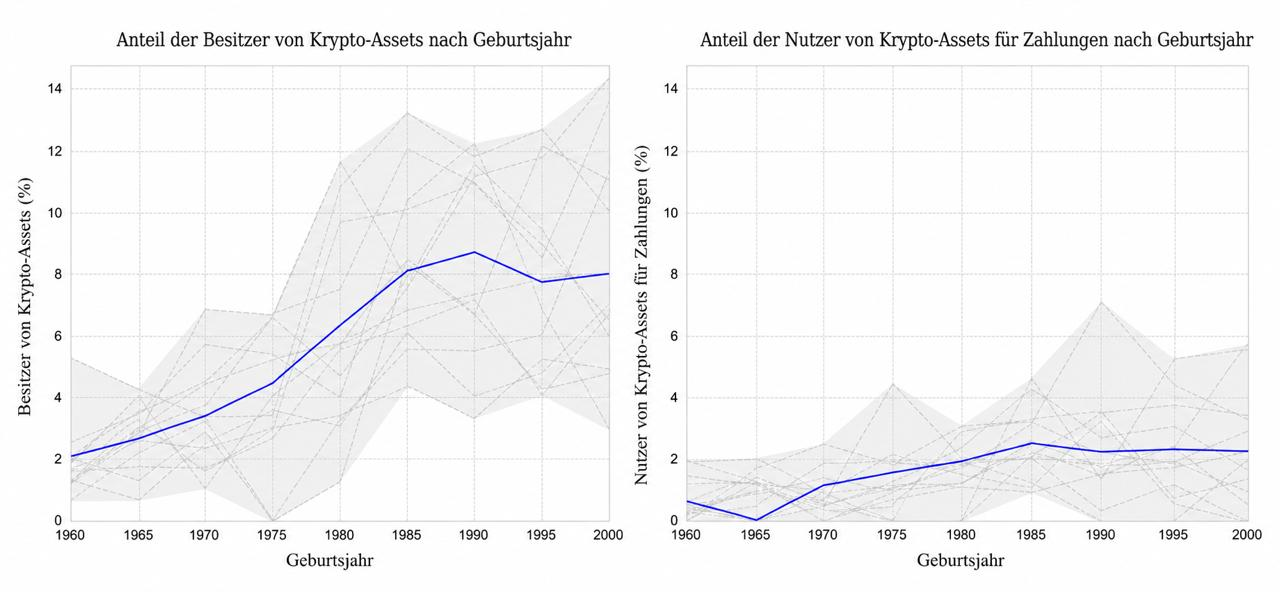
\includegraphics[width=0.98\textwidth]{img/eu/1.jpg}
    \caption{Krypto-Nutzung im Euroraum nach Geburtsjahr (2022) \cite{Zamora2026}.}
    \label{fig:krypto-besitz-zahlung-eu}
\end{figure}

Abbildung~\ref{fig:krypto-besitz-zahlung-eu} ist für die Forschungsfrage zentral. Sie zeigt, dass Kryptowährungen im Euroraum nicht unbekannt sind. Sie erfüllen jedoch nur begrenzt die Geldfunktion eines alltäglichen Zahlungsmittels. Viele Nutzer halten Krypto-Assets eher als Anlage oder Spekulationsobjekt. Dabei ist zu beachten, dass die Daten auf Selbstauskünften beruhen und nicht jede einzelne Transaktion messen \cite{Zamora2026}.

Fehlendes Vertrauen verstärkt diese Entwicklung. Für alltägliche Zahlungen erwarten Nutzer stabile Werte, einfache Bedienung, breite Akzeptanz im Handel und rechtliche Sicherheit. Kryptowährungen erfüllen diese Bedingungen im Euroraum nur teilweise. Deshalb werden sie zwar reguliert und teilweise als Vermögenswert gehalten, ersetzen aber nicht den Euro als allgemein akzeptiertes Zahlungsmittel.

\subsubsection{Zwischenfazit für die Forschungsfrage}

Der europäische Fall zeigt drei Gründe, warum Kryptowährungen bisher nicht als allgemein akzeptiertes Zahlungsmittel funktionieren. Erstens will der Staat die Kontrolle über Währung, Zahlungsverkehr und Finanzstabilität behalten. Zweitens werden Krypto-Assets wegen Risiken für Verbraucher und Marktintegrität reguliert, nicht als gesetzliches Zahlungsmittel eingeführt. Drittens fehlt im Alltag das Vertrauen, weil Preisstabilität, einfache Nutzung und Akzeptanz im Handel begrenzt bleiben. Die EU verbietet Kryptowährungen nicht, ordnet sie aber als regulierte Vermögenswerte ein und entwickelt mit dem digitalen Euro eine öffentliche digitale Alternative.

\endinput



